\documentclass[11pt]{article}
\usepackage[textwidth=18.0cm, textheight=23.0cm, top=2.0cm]{geometry}
\usepackage{pst-all}
\usepackage{amssymb}
\usepackage{tikz}
\usepackage{underscore}\begin{document}
\pagestyle{empty}


ClassName: \underline{\textbf{Class_08.2bp-7}}
\par
BinSize: \underline{\textbf{100 × 100}}
\par
ReduceSize: \underline{\textbf{100 × 100}}
\par
TypeNum: \underline{\textbf{20}}
\par
Num: \underline{\textbf{20}}
\par
OutS: \underline{\textbf{50000}}
\par
InS: \underline{\textbf{41921}}
\par
Rate: \underline{\textbf{0.838}}
\par
UB: \underline{\textbf{5}}
\par
LB0: \underline{\textbf{5}}
\par
LB: \underline{\textbf{5}}
\par
LBWithCut: \underline{\textbf{5}}
\par
NodeCut: \underline{\textbf{0}}
\par
ExtendedNodeCnt: \underline{\textbf{1}}
\par
GenNodeCnt: \underline{\textbf{1}}
\par
PrimalNode: \underline{\textbf{0}}
\par
ColumnCount: \underline{\textbf{5}}
\par
TotalCutCount: \underline{\textbf{0}}
\par
RootCutCount: \underline{\textbf{0}}
\par
LPSolverCnt: \underline{\textbf{1}}
\par
PricingSolverCnt: \underline{\textbf{0}}
\par
BranchAndBoundNum: \underline{\textbf{1}}
\par
isOpt: \underline{\textbf{true}}
\par
TimeOnInitSolution: \underline{\textbf{0.010 s}}
\par
TimeOnPrimal: \underline{\textbf{0.000 s}}
\par
TimeOnPricing: \underline{\textbf{0.000 s}}
\par
TimeOnRmp: \underline{\textbf{0.063 s}}
\par
TotalTime: \underline{\textbf{0.135 s}}
\par
\newpage


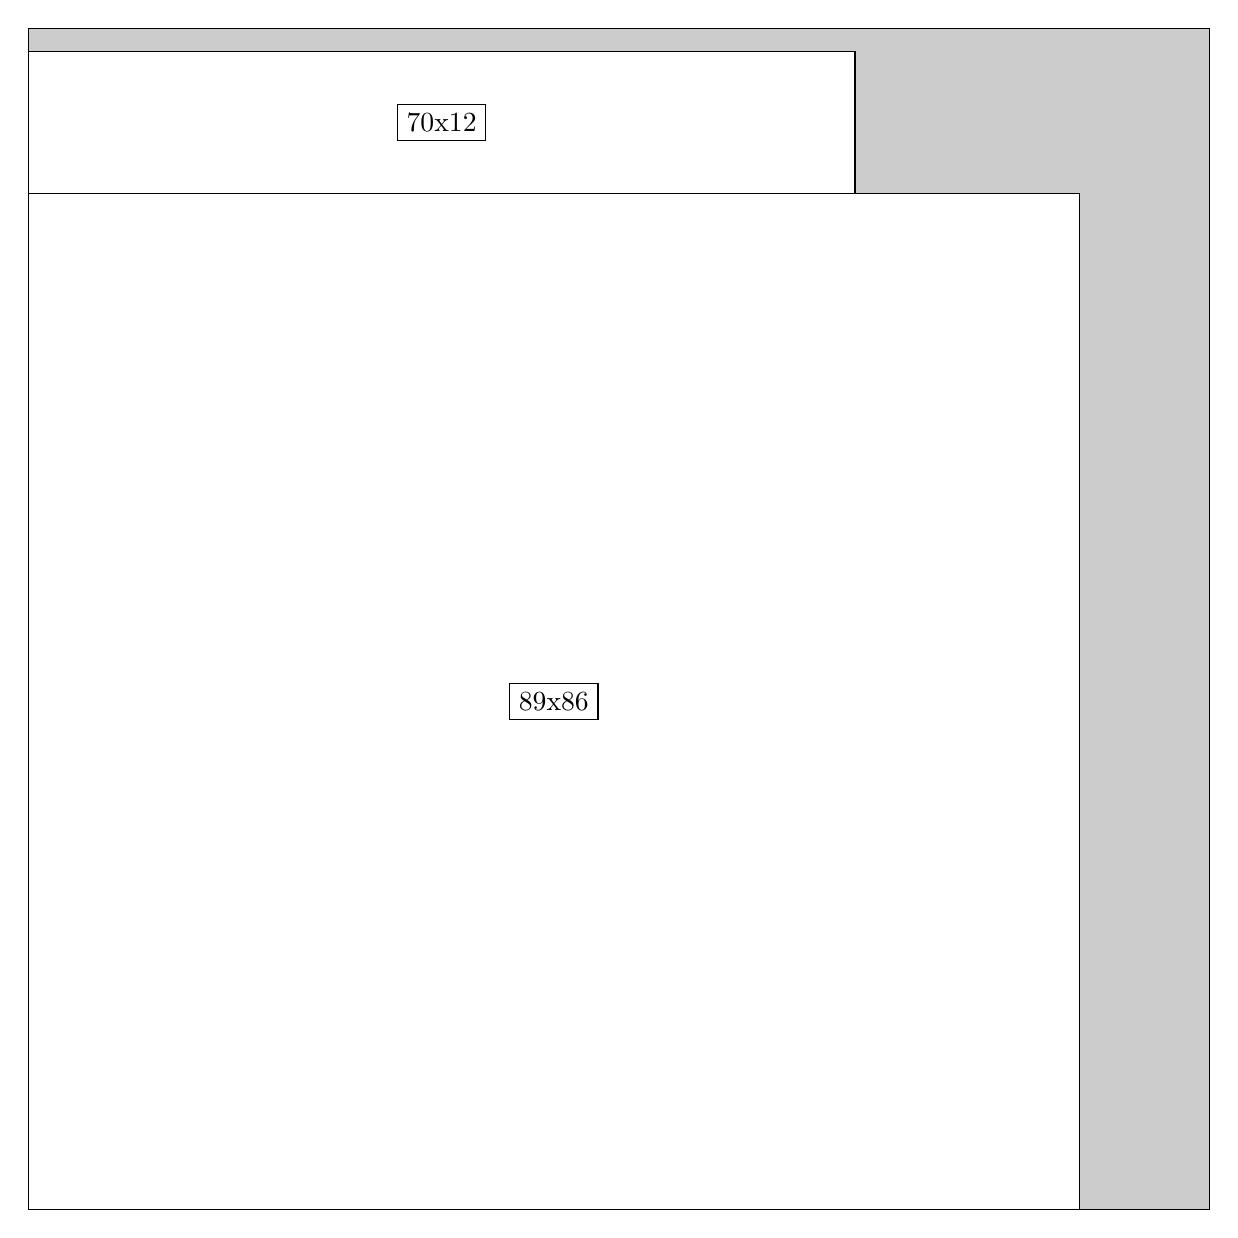
\begin{tikzpicture}[shorten >=1pt,scale=1.0,every node/.style={scale=1.0},->]
\tikzstyle{vertex}=[circle,fill=black!25,minimum size=14pt,inner sep=0pt]
\filldraw[fill=gray!40!white, draw=black] (0,0) rectangle (15.0,15.0);
\foreach \name/\x/\y/\w/\h in {89x86/0.0/0.0/13.35/12.9,70x12/0.0/12.9/10.5/1.7999999999999998}
\filldraw[fill=white!40!white, draw=black] (\x,\y) rectangle node[draw] (\name) {\name} ++(\w,\h);
\end{tikzpicture}


w =89 , h =86 , x =0 , y =0 , v =7654
\par
w =70 , h =12 , x =0 , y =86 , v =840
\par
\newpage


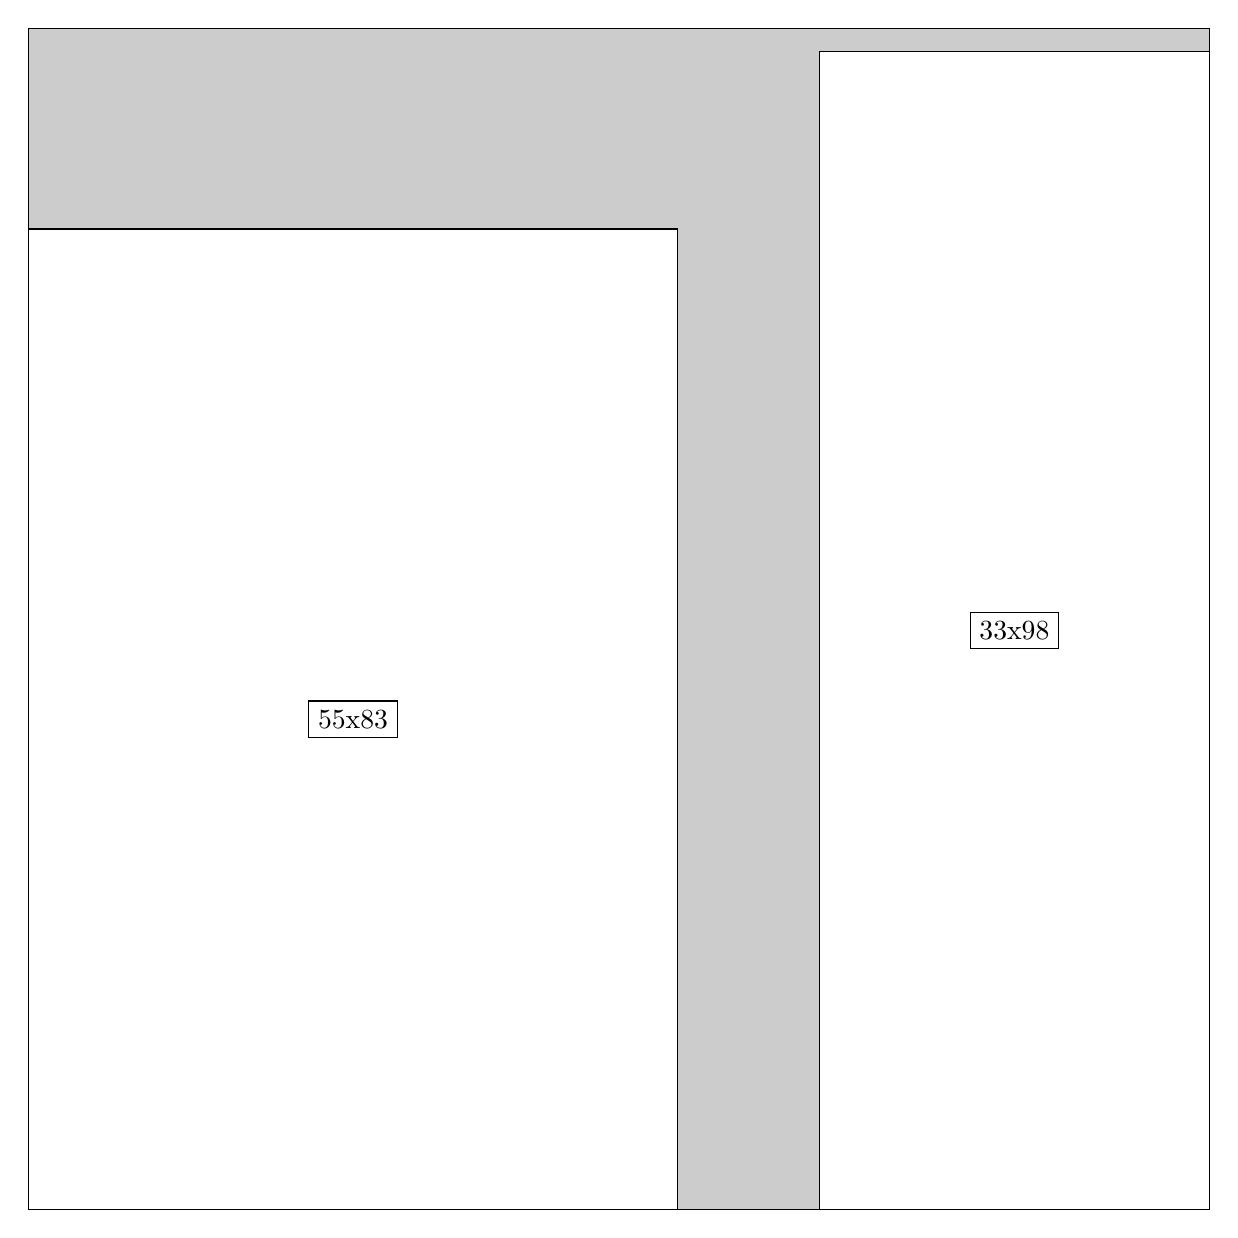
\begin{tikzpicture}[shorten >=1pt,scale=1.0,every node/.style={scale=1.0},->]
\tikzstyle{vertex}=[circle,fill=black!25,minimum size=14pt,inner sep=0pt]
\filldraw[fill=gray!40!white, draw=black] (0,0) rectangle (15.0,15.0);
\foreach \name/\x/\y/\w/\h in {55x83/0.0/0.0/8.25/12.45,33x98/10.049999999999999/0.0/4.95/14.7}
\filldraw[fill=white!40!white, draw=black] (\x,\y) rectangle node[draw] (\name) {\name} ++(\w,\h);
\end{tikzpicture}


w =55 , h =83 , x =0 , y =0 , v =4565
\par
w =33 , h =98 , x =67 , y =0 , v =3234
\par
\newpage


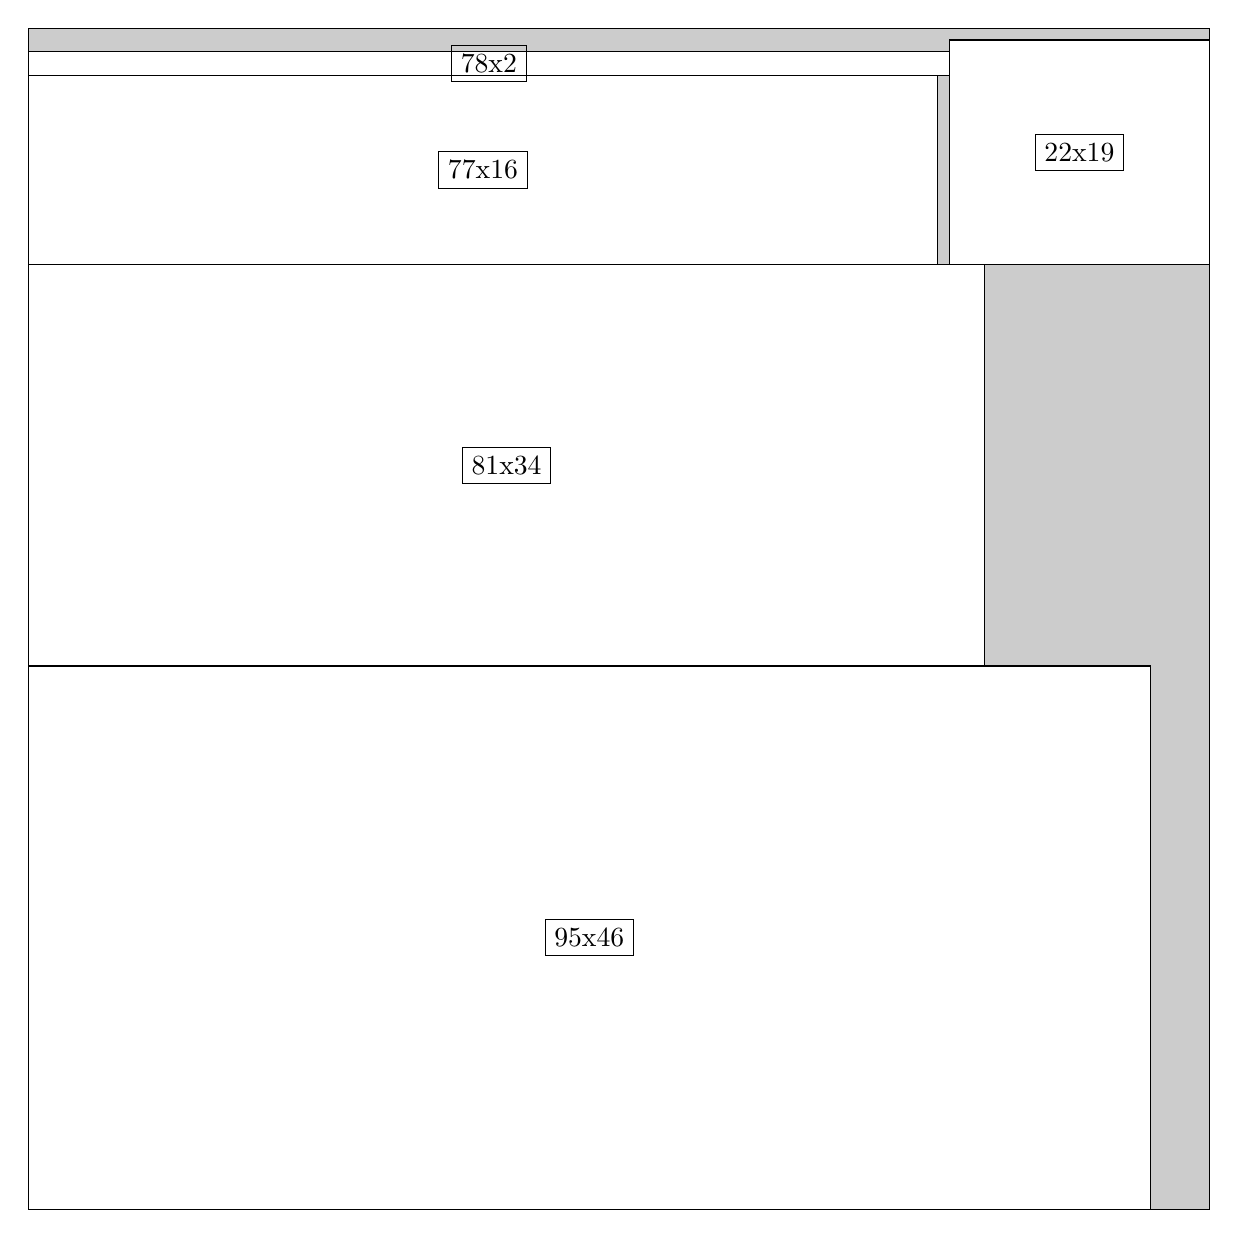
\begin{tikzpicture}[shorten >=1pt,scale=1.0,every node/.style={scale=1.0},->]
\tikzstyle{vertex}=[circle,fill=black!25,minimum size=14pt,inner sep=0pt]
\filldraw[fill=gray!40!white, draw=black] (0,0) rectangle (15.0,15.0);
\foreach \name/\x/\y/\w/\h in {95x46/0.0/0.0/14.25/6.8999999999999995,81x34/0.0/6.8999999999999995/12.15/5.1,77x16/0.0/12.0/11.549999999999999/2.4,22x19/11.7/12.0/3.3/2.85,78x2/0.0/14.399999999999999/11.7/0.3}
\filldraw[fill=white!40!white, draw=black] (\x,\y) rectangle node[draw] (\name) {\name} ++(\w,\h);
\end{tikzpicture}


w =95 , h =46 , x =0 , y =0 , v =4370
\par
w =81 , h =34 , x =0 , y =46 , v =2754
\par
w =77 , h =16 , x =0 , y =80 , v =1232
\par
w =22 , h =19 , x =78 , y =80 , v =418
\par
w =78 , h =2 , x =0 , y =96 , v =156
\par
\newpage


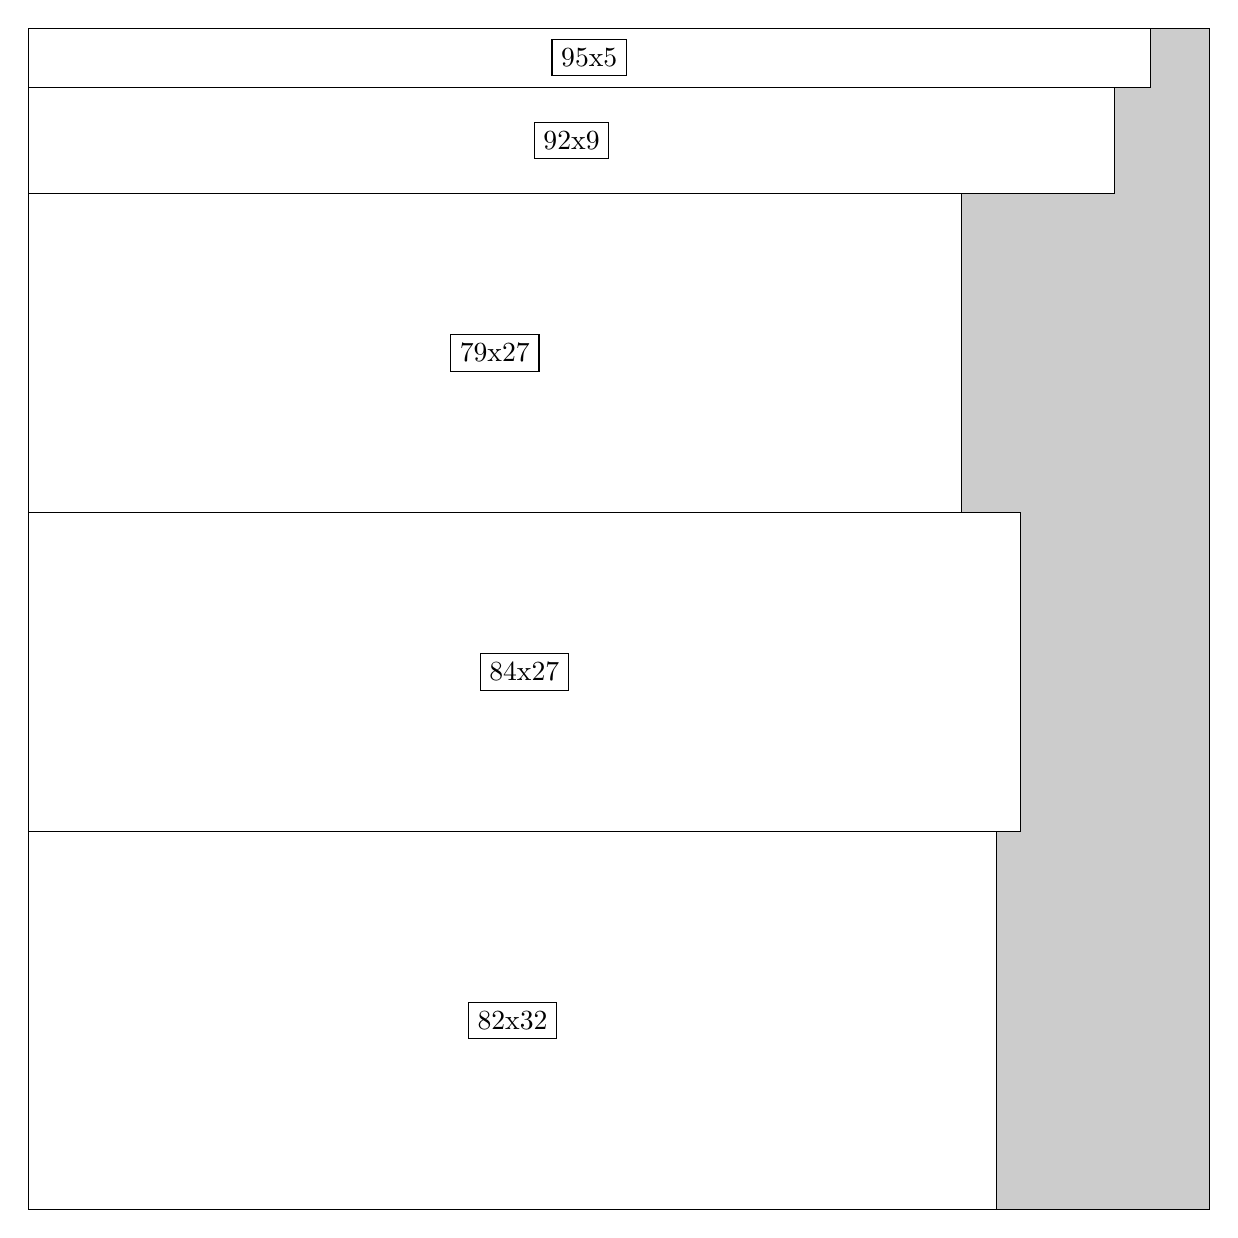
\begin{tikzpicture}[shorten >=1pt,scale=1.0,every node/.style={scale=1.0},->]
\tikzstyle{vertex}=[circle,fill=black!25,minimum size=14pt,inner sep=0pt]
\filldraw[fill=gray!40!white, draw=black] (0,0) rectangle (15.0,15.0);
\foreach \name/\x/\y/\w/\h in {82x32/0.0/0.0/12.299999999999999/4.8,84x27/0.0/4.8/12.6/4.05,79x27/0.0/8.85/11.85/4.05,92x9/0.0/12.9/13.799999999999999/1.3499999999999999,95x5/0.0/14.25/14.25/0.75}
\filldraw[fill=white!40!white, draw=black] (\x,\y) rectangle node[draw] (\name) {\name} ++(\w,\h);
\end{tikzpicture}


w =82 , h =32 , x =0 , y =0 , v =2624
\par
w =84 , h =27 , x =0 , y =32 , v =2268
\par
w =79 , h =27 , x =0 , y =59 , v =2133
\par
w =92 , h =9 , x =0 , y =86 , v =828
\par
w =95 , h =5 , x =0 , y =95 , v =475
\par
\newpage


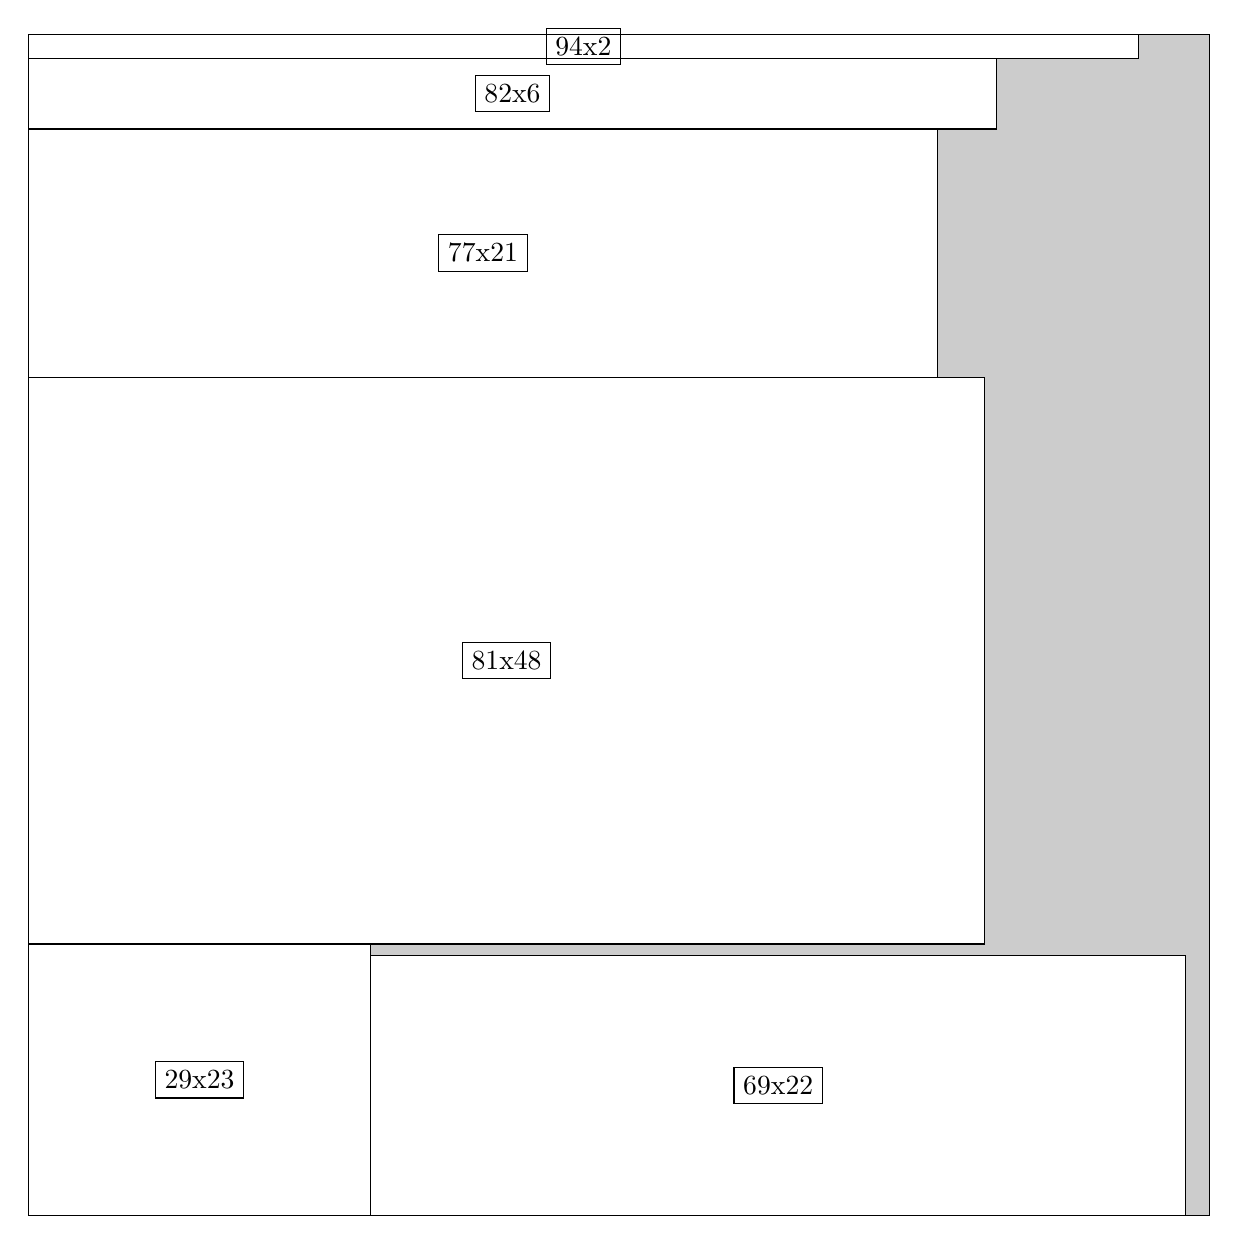
\begin{tikzpicture}[shorten >=1pt,scale=1.0,every node/.style={scale=1.0},->]
\tikzstyle{vertex}=[circle,fill=black!25,minimum size=14pt,inner sep=0pt]
\filldraw[fill=gray!40!white, draw=black] (0,0) rectangle (15.0,15.0);
\foreach \name/\x/\y/\w/\h in {29x23/0.0/0.0/4.35/3.4499999999999997,69x22/4.35/0.0/10.35/3.3,81x48/0.0/3.4499999999999997/12.15/7.199999999999999,77x21/0.0/10.65/11.549999999999999/3.15,82x6/0.0/13.799999999999999/12.299999999999999/0.8999999999999999,94x2/0.0/14.7/14.1/0.3}
\filldraw[fill=white!40!white, draw=black] (\x,\y) rectangle node[draw] (\name) {\name} ++(\w,\h);
\end{tikzpicture}


w =29 , h =23 , x =0 , y =0 , v =667
\par
w =69 , h =22 , x =29 , y =0 , v =1518
\par
w =81 , h =48 , x =0 , y =23 , v =3888
\par
w =77 , h =21 , x =0 , y =71 , v =1617
\par
w =82 , h =6 , x =0 , y =92 , v =492
\par
w =94 , h =2 , x =0 , y =98 , v =188
\par
\newpage


\end{document}